\chapter{Introducción}

\section{¿Qué es un fractal?}

La definición más inmediata que tenemos de los fractales es la siguiente:

\begin{definition}
    Un fractal es un objeto geométrico cuya estructura básica, fragmentada o irregular, se repite a diferentes escalas.
\end{definition}

\noindent Que su estructura básica se repita a diferentes escalas significa que el objeto es autosimilar.

\section{Autosimilitud}

Benoît Mandelbrot la definió como sigue:

\begin{definition}
    Un objeto es autosimilar o autosemejante si sus partes tienen la misma forma o estructura que el todo, aunque pueden presentarse a diferente escala y pueden estar ligeramente deformadas.
\end{definition}

\noindent
\large Vamos a ver dos tipos de autosimilitud:

\subsection{Autosimilitud exacta}

\begin{definition}
    Un objeto es exactamente autosimilar si es exactamente igual a sí mismo a diferentes escalas..
\end{definition}

\noindent
Es la más restrictiva de todas y la que vemos en los fractales clásicos. Algunos ejemplos de objetos exactamente autosimilares son:

\begin{itemize}
    \item El triángulo de Sierpinski
    
    \begin{figure}[H]
        \centering
        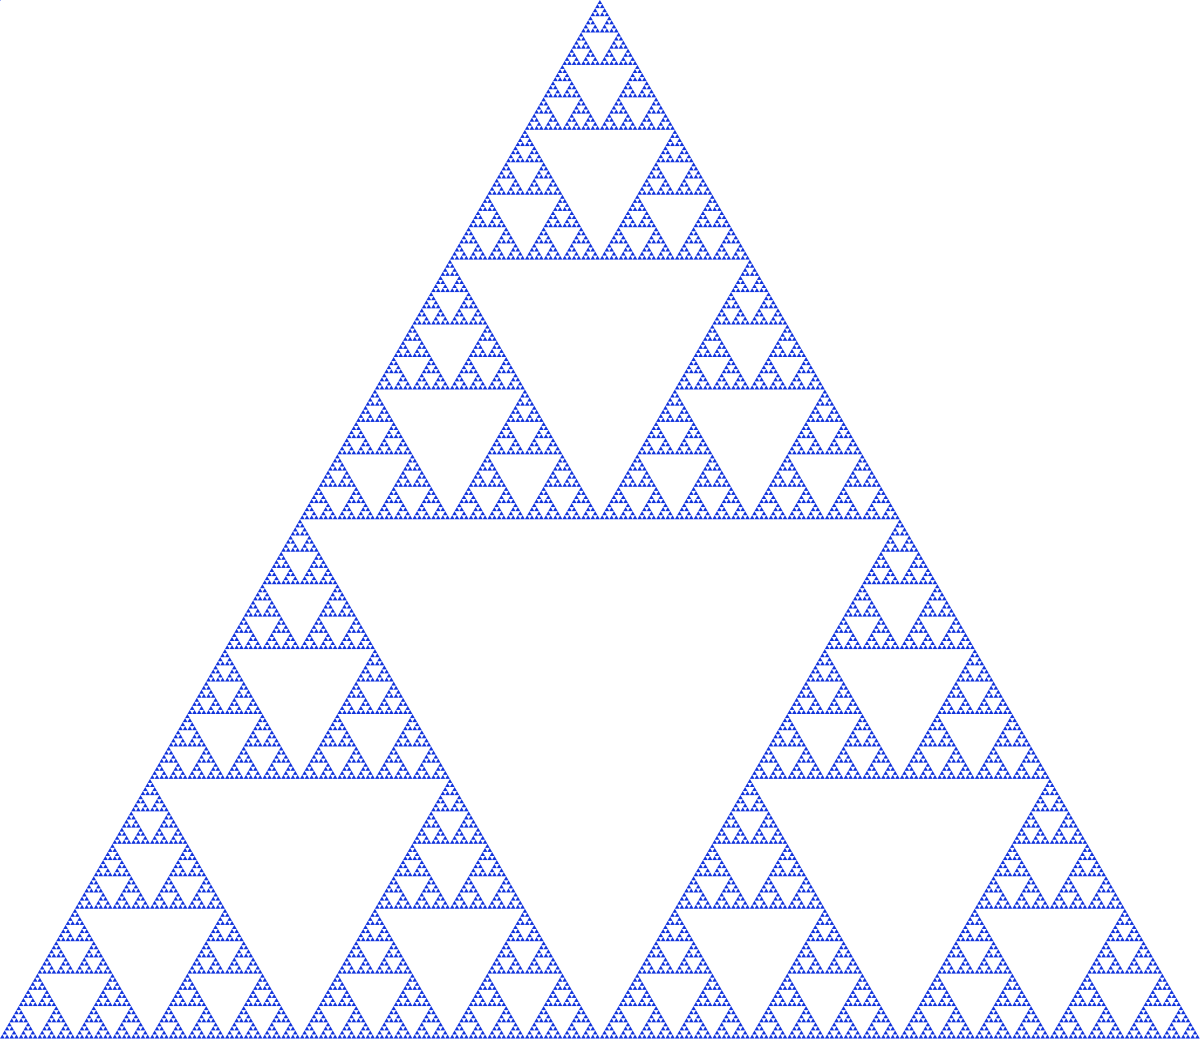
\includegraphics[width=0.5\textwidth]{figures/sierpinski-triangle.png}
        \caption{Triángulo de Sierpinski}
    \end{figure}

    \item El copo de Koch
    
    \begin{figure}[H]
        \centering
        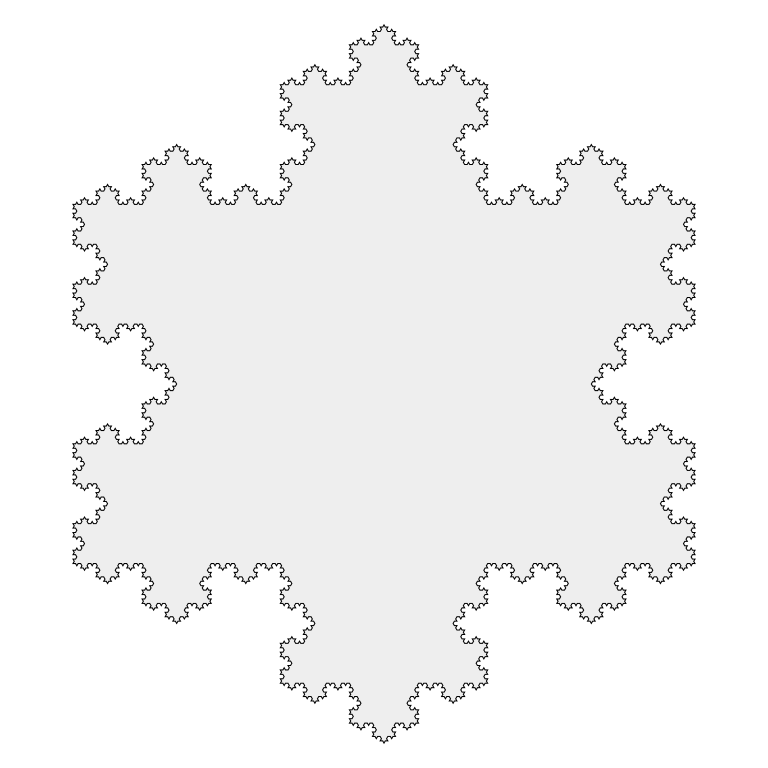
\includegraphics[width=0.5\textwidth]{figures/koch-snowflake.png}
        \caption{Copo de Koch}
    \end{figure}

\end{itemize}

\subsection{Cuasiautosimilitud}

\begin{definition}
    Un objeto es cuasiautosimilar si es aproximadamente igual a sí mismo a diferentes escalas.
\end{definition}

\noindent
Los fractales de este tipo contienen copias menores y distorsionadas de si mismos, como occure por ejemplo con el conjunto de Mandelbrot.

\begin{figure}[H]
    \centering
    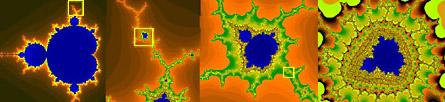
\includegraphics[width=0.7\textwidth]{figures/mandelbrot-cuasi.png}
    \caption{Ejemplos de cuasiautosimilitud en el conjunto de Mandelbrot}
\end{figure}


\section{Definición más formal}

\noindent En 1982 Benoît Mandelbrot definió los fractales de la siguiente forma:

\begin{definition}
Un fractal es un conjunto cuya dimensión de Hausdorff-Besicovitch es estrictamente mayor que su dimensión topológica.
\end{definition}

\noindent La dimesión topológica es la dimensión que todos conocemos, la dimensión de Hausdorff-Besicovitch es una generalización de la dimensión topológica que nos permite calcular la dimensión de conjuntos que no son enteros, como por ejemplo el conjunto de Cantor.

\section{Dimensión fractal}